\documentclass{article}
\usepackage[brazilian]{babel}
\usepackage[utf8]{inputenc}
\usepackage[T1]{fontenc}
\usepackage{listings}
\usepackage{xcolor}
\usepackage{graphicx}
\usepackage{geometry}


\geometry{
  a4paper,
  total={170mm,257mm},
  left=25mm,
  top=20mm,
  }

\graphicspath{ {./images/} }



\author{
  Mauricio Ramos Ribeiro\\
  \texttt{mauricio.ribeiro@outlook.com.br}
}


\title{Respostas dos Exercícios de Arranjos}
\date{\today}

\begin{document}
\maketitle

\vspace{15mm}


\section*{Questão 1:}
\lstinputlisting[language=C++, firstline=1]{../1.dupeliminate/src/main.cpp}
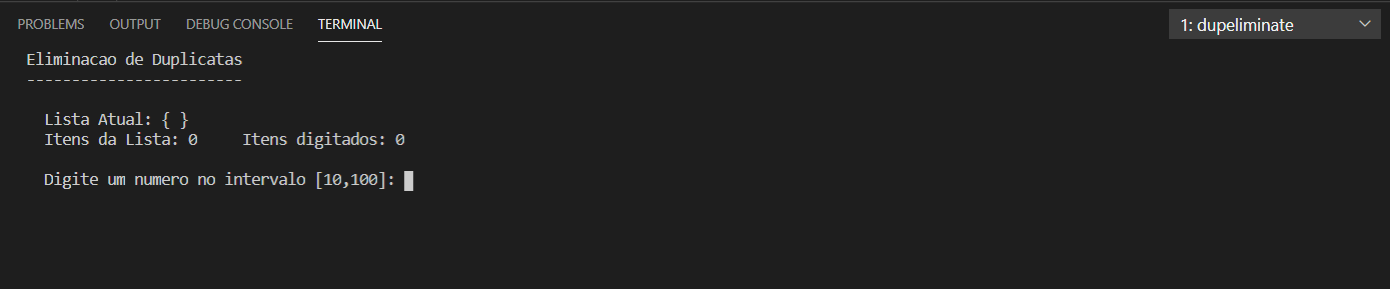
\includegraphics[scale=0.6]{01.1.png}

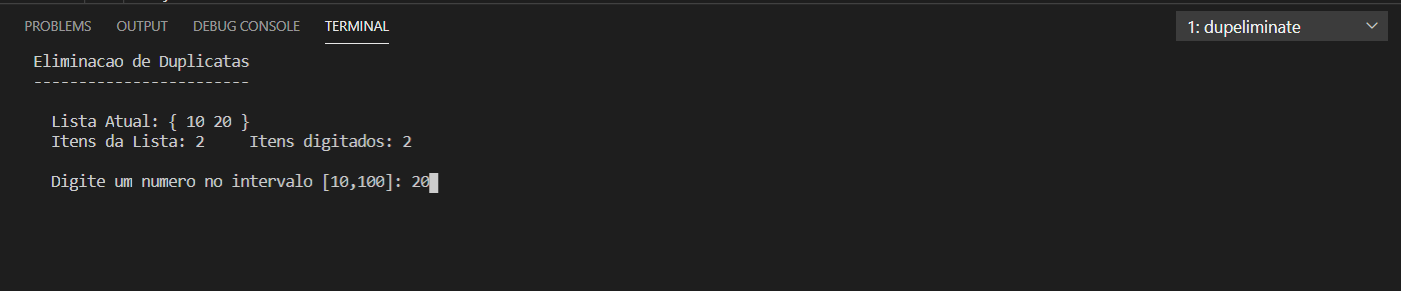
\includegraphics[scale=0.6]{01.2.png}

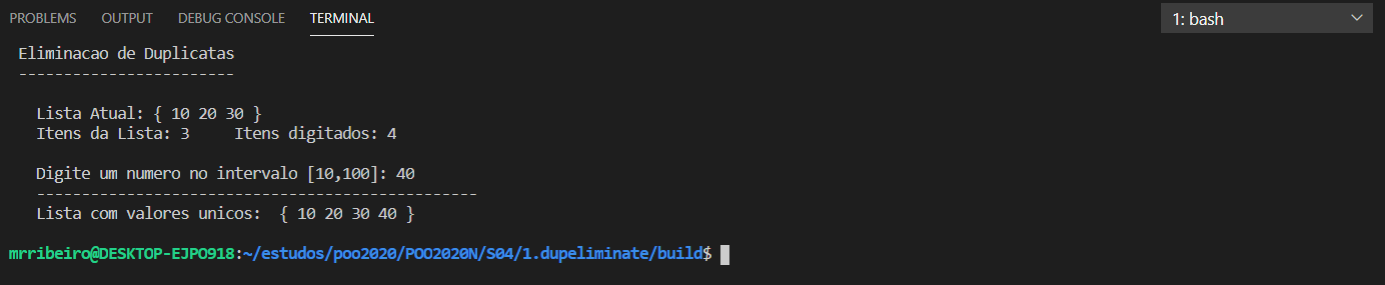
\includegraphics[scale=0.6]{01.3.png}
\vspace{15mm}



\end{document}